\section{Méthodologie}
\begin{frame}
    \frametitle{Étapes de la Méthodologie}
    \begin{figure}
        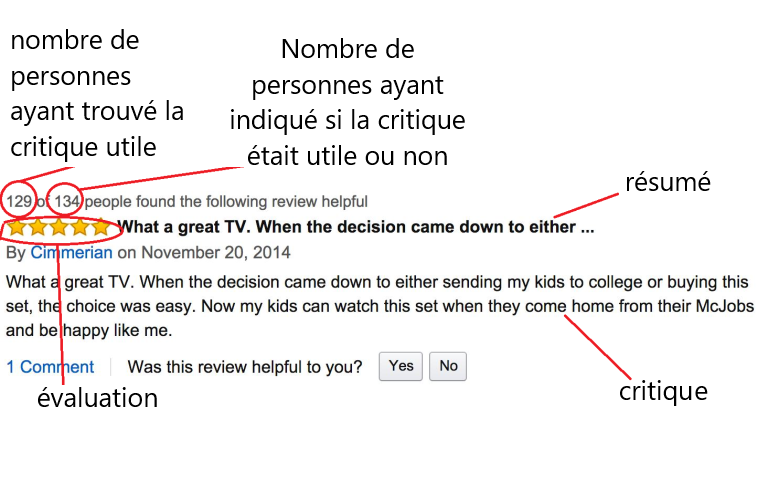
\includegraphics[scale=0.3]{Figures/amazonReviewDetails.png}
        \caption{Les elements d’un avis}
    \end{figure}
\end{frame}
\begin{frame}
    \begin{enumerate}
        \item \textbf{Collecte de Données} :
            \begin{itemize}
                \item Collecte des avis sur les produits alimentaires d'Amazon.
                \item Utilisation de la fonction \texttt{data.info()} pour examiner la structure de l'ensemble de données.
            \end{itemize}
        \item \textbf{Informations Générales sur la Dataset} :
            \begin{itemize}
                \item Utilisation de la fonction \texttt{data.info()} pour obtenir une vue détaillée de la structure de l'ensemble de données.
                \item Analyse des attributs et types de données de chaque colonne.
            \end{itemize}
    \end{enumerate}
    \begin{figure}[h]
    \centering
    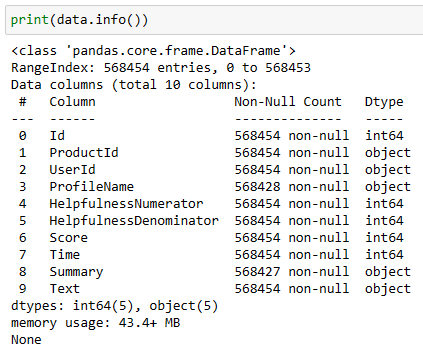
\includegraphics[scale=0.35]{Figures/datainfo.PNG}
    \caption{Les information sur la DataSet}
    \label{fig:dataframeinfo}
\end{figure}
\end{frame}


\begin{frame}
    \frametitle{Étapes de la Méthodologie (suite)}

    \begin{enumerate}
        \setcounter{enumi}{2}
        \item \textbf{Statistiques Descriptives pour les Attributs Numériques} :
            \begin{itemize}
                \item Utilisation de la commande \texttt{data['Score'].describe()} pour obtenir des statistiques descriptives pour l'attribut "Score".
            \end{itemize}
            \begin{figure}[h]
                \centering
                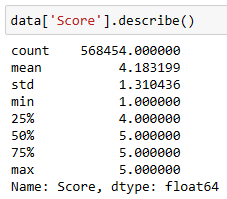
\includegraphics[scale=0.5]{Figures/describe.PNG}
                \caption{Statistiques descriptives pour l'attribut Score}
                \label{fig:describe}
            \end{figure}
    \end{enumerate}

    \begin{enumerate}
        \setcounter{enumi}{3}
        \item \textbf{Vérification des Valeurs Manquantes ou d'Incohérences} :
            \begin{itemize}
                \item Utilisation de la commande \texttt{data.isnull().sum()} pour détecter les valeurs manquantes dans chaque colonne.
            \end{itemize}
    \end{enumerate}
\end{frame}

\begin{frame}
    \frametitle{Étapes de la Méthodologie (suite)}

    \begin{enumerate}
        \setcounter{enumi}{4}
        \item \textbf{Vérifier les Valeurs Uniques dans Chaque Colonne} :
            \begin{itemize}
                \item Utilisation de la commande \texttt{data.nunique()} pour explorer la diversité des valeurs dans chaque colonne.
                \item Interprétation des résultats.
            \end{itemize}
        \item \textbf{Prétraitement des Données} :
            \begin{itemize}
                \item Élimination des lignes en double et gestion des valeurs manquantes avec \texttt{data.drop\_duplicates()} et \texttt{data.dropna()}.
            \end{itemize}
    \end{enumerate}
\end{frame}

\begin{frame}
    \begin{enumerate}
        \setcounter{enumi}{6}
        \item \textbf{Analyse Exploratoire des Données} :
            \begin{itemize}
                \item Distribution des scores.
                \begin{figure}[h]
                    \centering
                    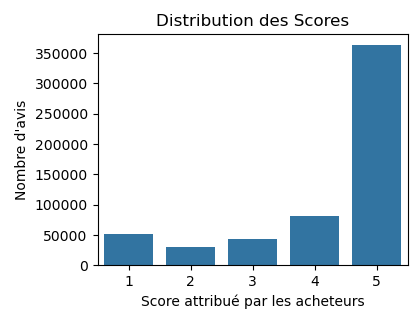
\includegraphics[width=0.7\linewidth]{Figures/distrubutiondesscores.PNG}
                    \captionsetup{font=scriptsize}
                    \caption{La distribution des scores}
                    \label{fig:distribution_des_scores}
                \end{figure}
            \end{itemize}
    \end{enumerate}
\end{frame}

\begin{frame}
    \begin{enumerate}
        \setcounter{enumi}{6}
        \item \textbf{Analyse Exploratoire des Données} :
            \begin{itemize} 
                \item Calcul de la moyenne et de la médiane des scores.
                \[
                \text{Moyenne des scores : } 4.18
                \]
                \[
                \text{Médiane des scores : } 5.0
                \]
            \end{itemize}
    \end{enumerate}
\end{frame}

\begin{frame}
    \begin{enumerate}
        \setcounter{enumi}{6}
        \item \textbf{Analyse Exploratoire des Données} :
            \begin{itemize}
                \item Distribution des sentiments.
                \begin{figure}[h]
                    \centering
                    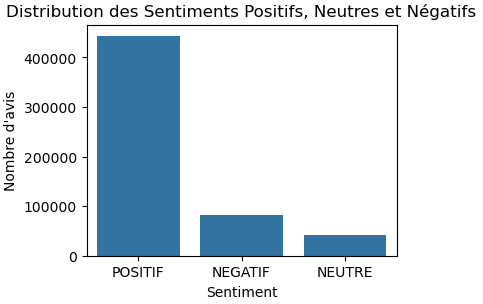
\includegraphics[width=0.7\linewidth]{Figures/distrubutiondessentiments.PNG}
                    \captionsetup{font=scriptsize}
                    \caption{Distribution des Sentiments}
                    \label{fig:distribution_des_sentiments}
                \end{figure}
            \end{itemize}
    \end{enumerate}
\end{frame}



\begin{frame}
    \frametitle{Étapes de la Méthodologie (suite)}

    \begin{enumerate}
        \setcounter{enumi}{7}
        \item \textbf{Traitement du Texte} :
            \begin{itemize}
                \item Suppression des URL, des balises HTML, des caractères non alphabétiques.
                \item Conversion en minuscules et suppression des stopwords.
            \end{itemize}
        \item \textbf{Utilisation du Modèle Pré-entraîné RoBERTa} :
            \begin{itemize}
                \item Initialisation du modèle RoBERTa et du tokenizer.
                \item Fonction d'évaluation des scores de RoBERTa pour l'analyse de sentiments.
                \item Analyse de sentiments avec RoBERTa sur l'ensemble de données.
            \end{itemize}
        \item \textbf{Transformation et Fusion des Résultats} :
            \begin{itemize}
                \item Stockage des résultats du modèle avec les données d'origine.
                \item Exportation des résultats en CSV (\texttt{nlp\_results.csv}).
            \end{itemize}
    \end{enumerate}
\end{frame}
